\section{Anhang}
\begin{appendix}

\section{Versuchsprotokoll}

\begin{figure}[H]
\centering 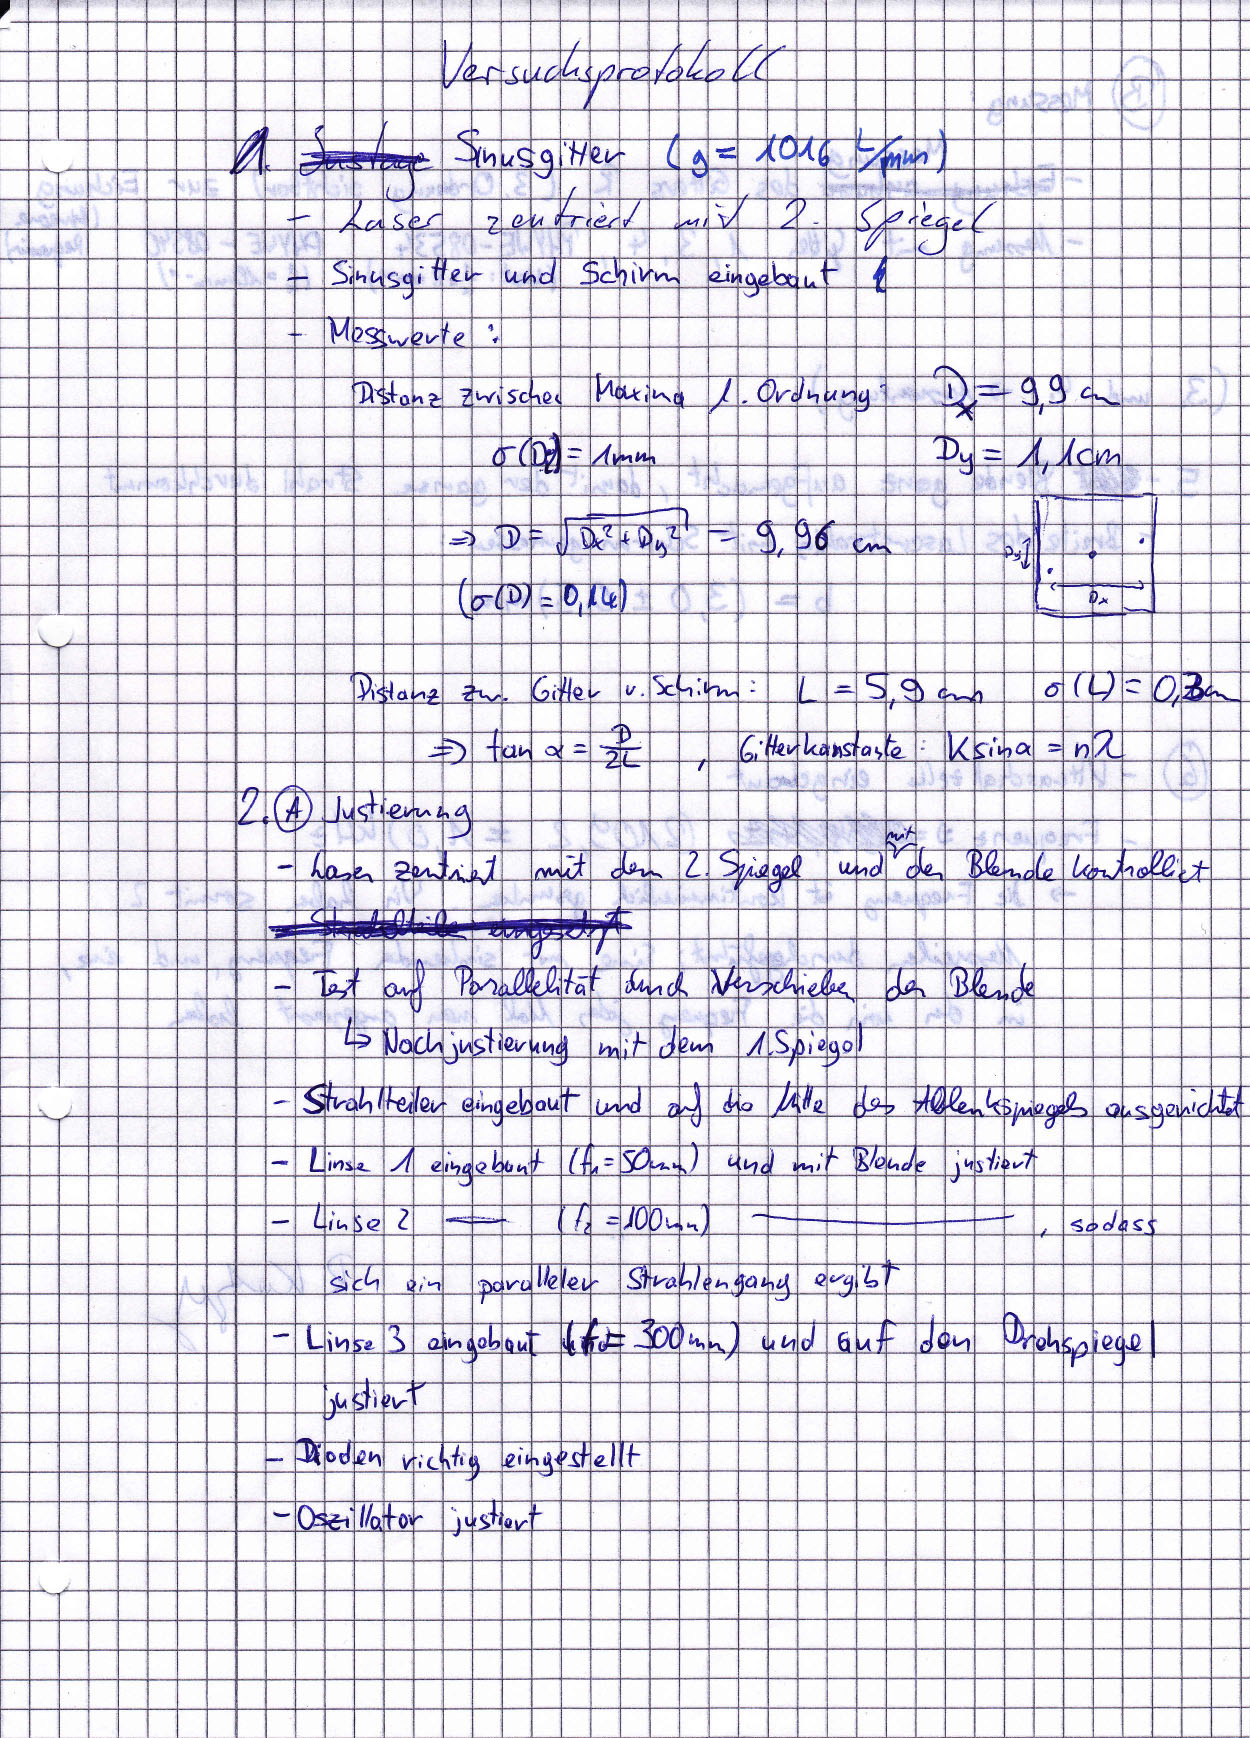
\includegraphics[width=\textwidth]{Bilder/Protokoll1.jpg}
\end{figure}

\clearpage


\begin{figure}[H]
\centering 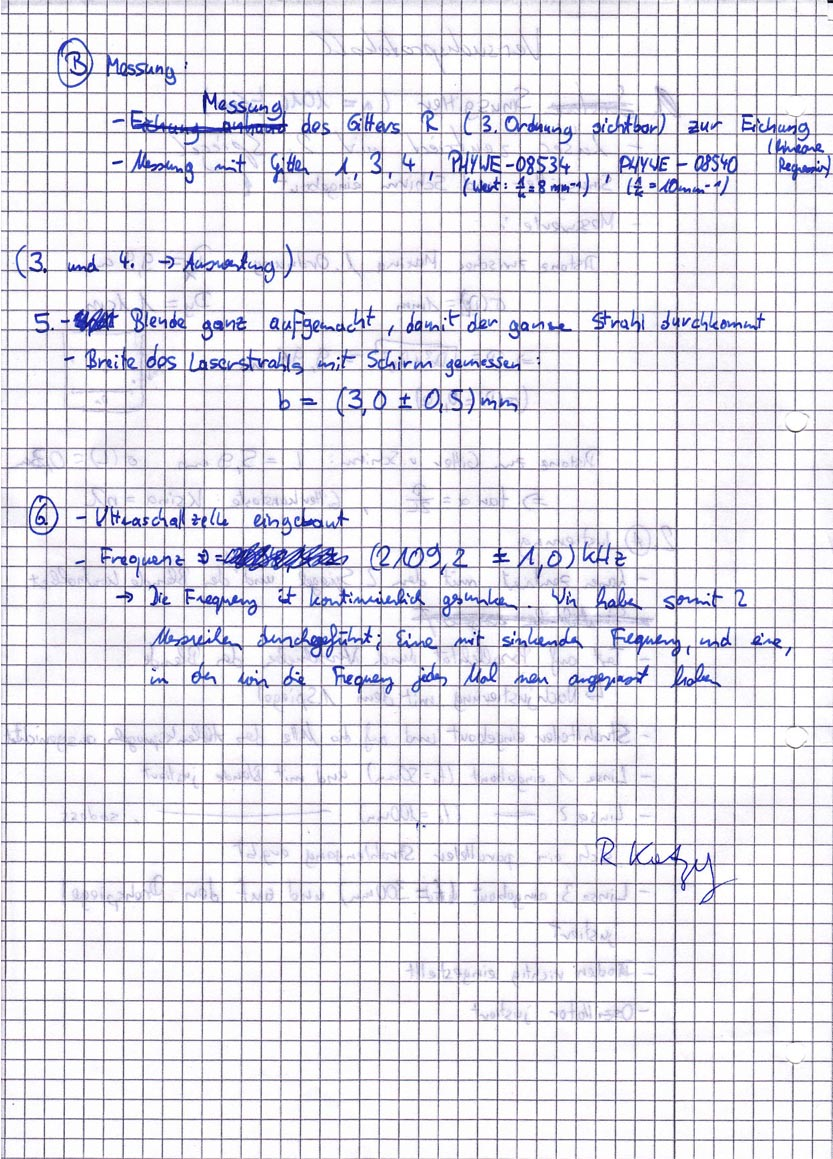
\includegraphics[width=\textwidth]{Bilder/Protokoll2.jpg}
\end{figure}

\section{Messwerte}

\subsection[Intensität der Maxima]{Intensität der Maxima bei der Ultraschallzelle}

Die abgelesenen Werte sind in der Form:
"`werte[Spannung in V][Ordnung] = Intensität in V; s[Spannun][Ordnung] = Fehler auf die Intensität;"'

\begin{verbatim}
 werte[0.0][0] = 7.81411; s[0][0] = 0.05;
  werte[0.0][1] = 0.534180; s[0][1] = 0.05;
  werte[0.0][2] = 0.165152; s[0][2] = 0.05;
  
  werte[1.01][0] = 7.58345; s[1.01][0] = 0.05;
  werte[1.01][1] = 0.595606; s[1.01][1] = 0.05;

  werte[2.0][0] = 7.18386; s[2][0] = 0.05;
  werte[2.0][1] = 0.911210; s[2][1] = 0.05;
  
  werte[3.0][0] = 6.65979; s[3.0][0] = 0.05;
  werte[3.0][1] = (0.988260 + 1.06716) /2; s[3.0][0] = 0.03 / sqrt(2.);
  
  werte[3.99][0] = 5.90614; s[3.99][0] = 0.04;
  werte[3.99][1] = (1.32051 + 1.37895) / 2; s[3.99][1] = 0.01 / sqrt(2.);
  werte[3.99][2] = 0.1459; s[3.99][2] = 0.04;
  
  werte[4.99][0] = 5.10557; s[4.99][0] = 0.05;
  werte[4.99][1] = (1.67044 + 1.71344) / 2; s[4.99][1] = 0.05 / sqrt(2.);
  werte[4.99][2] = 0.232797; s[4.99][2] = 0.1;
  
  werte[5.66][0] = 4.46693; s[5.66][0] = 0.04;
  werte[5.66][1] = ( 1.98781 + 1.98498)/ 2; s[5.66][1] = 0.04 / sqrt(2);
  werte[5.66][2] = 0.307564; s[5.66][2] = 0.04;
  
  werte[6.34][0] = 3.76185; s[6.34][0] = 0.02;
  werte[6.34][1] = (2.18152 + 2.20363) /2; s[6.34][1] = 0.03 / sqrt(2);
  werte[6.34][2] = (0.366363 + 0.345704) / 2; s[6.34][2] = 0.03 / sqrt(2);
  
  werte[7.00][0] = 3.16188; s[7][0] = 0.02;
  werte[7.00][1] = (2.40147 + 2.40510) / 2; s[7][1] = 0.03 /sqrt(2);
  werte[7.00][2] = (0.482917 + 0.445933) / 2; s[7][2] = 0.03 / sqrt(2);
  
  werte[7.68][0] = 2.58162; s[7.68][0] = 0.03;
  werte[7.68][1] = (2.56090+2.54017)/2; s[7.68][1] = 0.03 / sqrt(2);
  werte[7.68][2] = (0.604586+0.558788) / 2; s[7.68][2] = 0.03 / sqrt(2);
  
  werte[8.33][0] = 1.64141; s[8.33][0] = 0.03;
  werte[8.33][1] = (2.76328 + 2.72248)/2; s[8.33][1] = 0.02 / sqrt(2);
  werte[8.33][2] = (0.819292 + 0.782161)/2; s[8.33][2] = 0.03 / sqrt(2);
  werte[8.33][3] = (0.162417 + 0.121085)/2; s[8.33][3] = 0.03 / sqrt(2);
  
  werte[8.99][0] = 1.20705; s[8.99][0] = 0.03;
  werte[8.99][1] = (2.74320 + 2.74059 )/2; s[8.99][1] = 0.03 / sqrt(2);
  werte[8.99][2] = (0.985601 + 0.887822 ) / 2; s[8.99][2] = 0.03 / sqrt(2);
  werte[8.99][3] = (0.177135 + 0.139159 ) / 2; s[8.99][3] = 0.03 / sqrt(2);
  
  werte[9.69][0] = 0.970063; s[9.69][0] = 0.04;
  werte[9.69][1] = (2.65724 + 2.66896)/2; s[9.69][1] = 0.03 / sqrt(2);
  werte[9.69][2] = (1.10564 +  1.04613) / 2; s[9.69][2] = 0.04 / sqrt(2);
  werte[9.69][3] = (0.231922 +  0.189630) / 2; s[9.69][3] = 0.04 / sqrt(2);
\end{verbatim}

\end{appendix}